\chapter{Implementierung}
\label{ch:methode}

In Kapitel \ref{ch:theorie} wurde das theoretisch-mathematische Modell beschrieben, mit welchem ein Bit geschrieben und wieder rekonstruiert werden kann. Um dieses Wissen nun praktisch nutzen zu können wurde ein Framework ausgearbeitet in dem es zur Anwendung kommt. 

\section{Architektur}

Das von Shannon und Weaver entwickelte Sender-Empfänger-Modell \cite{shannon2001mathematical} kann herangezogen werden, um den Aufbau des Kommunikationssystems zu modellieren:

\begin{figure}[h]
	\centering
	%\includesvg[width=0.7\textwidth]{figures/diagram-framework.svg}
	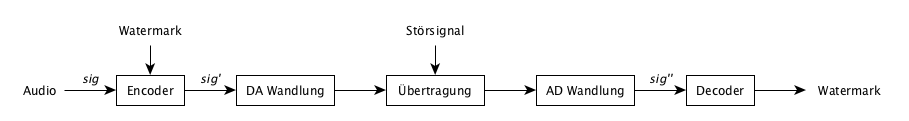
\includegraphics[width=0.9\textwidth]{figures/diagram-framework.png}
	\caption{Das Framework im Kommunikationsprozess}
	\label{fig:diagram-framework}
\end{figure}

Ein beliebiges digitales Signal soll mit einer Information, dem \textit{Watermark}\index{Watermark}, angereichert werden. Das Encodermodul verflechtet basierend auf der Grundlage von Kapitel \ref{sec:embeddingstragety_bitsequence} das Watermark mit dem Signal und liefert erneut ein digitales Signal.

Wir das neue digitale Signal auf analoger Ebene übertragen, muss eine DA-Wandlung\index{DA-Wandlung} vorgenommen werden. In der Regel wird das Signal über ein Lautsprechersystem abgespielt werden. Allerdings ist auch die reine Übertragung von einer Soundkarte zu einer anderen via einem Audiokabel eine DA-Wandlung. Ebenso würde das Pressen einer Schallplatte oder das Übertragen auf ein analoges Tonband in diese Kategorie fallen. 

Jede analoge Übertragung geschieht auf einem analogen Trägermedium, da Schall nicht im leeren Raum existieren kann, sondern sich auf einem Medium ausbreiten muss. Für den menschlichen Hörapparat ist dies normalerweise die Luft. Aber auch in Wasser kann sich Schall ausbreiten\footnote{Hier sogar viel besser. Viele Meereslebewesen nutzen diesen Umstand sehr stark aus, da sich Licht unter Wasser nur wenige 100 Meter ausbreitet. Auch das Sonar basiert darauf.} sowie in Festkörpern. In letzteren liegt oftmals das Signal nicht direkt als Schallwelle vor, sondern im Falle eines Audiokabels etwa als elektrisches Signal. 

Doch egal welches Medium benutzt wird, jeder Übertragungskanal\index{\"Ubertragungskanal} verändert das Signal durch seine Umwelteinflüsse während es ihn durchläuft. In der Luft etwa kommen die übrigen Geräusche der Umgebung hinzu, u.a. auch die Eigenreflexion der Schallwelle an der Umgebung. 
Wir wollen uns mit den diversen Formen und Ursachen von Störsignalen nicht näher befassen. Für uns ist wichtig, dass jede Störung das Signal verändert. Das mit Informationen angereicherte, modifizierte Signal überlagert sich also mit den Störungen. Dies wird sich in der Regel negativ auf das Watermark\index{Watermark} auswirken. 

Um das Watermark rekonstruieren zu können, muss das Signal zuerst wieder in eine digitale Form gebracht werden. Dies geschieht durch eine AD-Wandlung\index{AD-Wandlung}. Eine Schallwelle wird durch ein Mikrofon aufgenommen, ein elektrisches Signal durch den Line-in Eingang einer Soundkarte umgewandelt. 

Das Decodermodul versucht anschließend, das Watermark\index{Watermark} zu rekonstruieren. Hier gilt es zwei Probleme zu überwinden. Erstens muss das Watermark erkannt werden, d.h. der Decoder muss herausfinden wo eingebettete Daten sind. Dazu werden wir sog. \textit{Synchronisations-Codes} mit speziellen Eigenschaften bemühen (näheres in Abschnitt \ref{sec:barker-code}). Und zweitens müssen die eingeflochtenen Bits wieder \textit{richtig} rekonstruiert werden. Aufgrund des Störsignals welches im Übertragungskanal\index{\"Ubertragungskanal} das Signal in Mitleidenschaft zieht kann sich dies durchaus als schwierig herausstellen. Zur Erhöhung der Resistenz werden in Abschnitt \ref{sec:errorcorrection} Fehlerkorrekturverfahren\index{Fehlerkorrekturverfahren} eingeführt. Es sei allerdings an dieser Stelle bereits darauf hingewiesen, dass das Signal im Allgemeinen so weit deformiert werden kann, dass auch die Fehlerkorrektur eine sowohl vollständige wie auch richtige Rekonstruktion nicht gewährleisten kann. 

\section{Watermark Implantierung}
\label{sec:embedding}
\index{Watermark}

Der Implantationsprozess wird schematisch in Abbildung \ref{fig:diagram-encoder} modelliert. Ein anzureicherndes digitales Audiosignal wird zunächst in gleich große Bereiche segmentiert, d.h. die Samples des Signals werden in Gruppen zu je $N_s$\index{Sample-Section-Length} Samples zerteilt. In jede Gruppe (sog. \textit{Sample Section}\index{Sample Section}) wird genau 1 Bit kodiert. Der Einbettungsprozess geschieht in der DWT-Domain, daher werden die DWT-Koeffizienten \index{DWT-Koeffizienten} der Sample Section berechnet (eine Samples Section besteht aus einer Reihen aufeinander folgender Messpunkte eines Signal - sie beschreiben also einen Teil eines Signal und können ganz einfach wieder als eigenständiges Signal betrachtet werden). 

\begin{figure}[h]
	\centering
	%\includesvg[width=0.7\textwidth]{figures/diagram-framework.svg}
	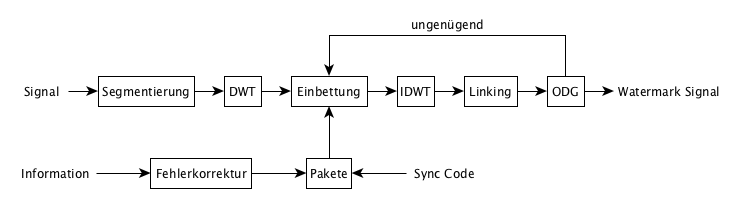
\includegraphics[width=\textwidth]{figures/diagram-encoder-v2.png}
	\caption{Schematischer Aufbau des Implemetierungsprozesses}
	\label{fig:diagram-encoder}
\end{figure}

Jede Sample Section\index{Sample Section} bekommt ein Bit der Bitsequenz, die das Signal beherbergen soll. Diese Sequenz setzt sich zusammen aus einer Kombination der mit Redundanz angereicherten (Abschnitt \ref{sec:errorcorrection}) eigentlichen Informationen und der Synchronisation-Codes\index{Synchronisations-Code}. Die Einbettung jedes Bit geschieht nach dem in Abschnitt \ref{sec:embeddingstragety} beschriebenen Algorithmus durch Veränderung der DWT-Koeffizienten\index{DWT-Koeffizienten}. Um das neue angereicherte Signal nun herzustellen werden auf die DWT-Koeffizienten eine inverse DWT-Transformation (IDWT)\index{inverse DWT-Transformation} angewandt. Diese resultiert in einer neuen Samples Section. Diese ersetzen im neuen Signal die unimplantierten Samples der korrelierenden Sample Section. 

Um sicherzustellen, dass das Watermark\index{Watermark} unhörbar in die Sample Section\index{Sample Section} implantiert wurde, wird noch eine Qualitätskontrolle vorgenommen. Dazu wird für ein Signalstück der sog. \textit{Objective Difference Grade} (ODG) berechnet. Erfüllt dieser einen vorgegebenen Grenzwert, so ist das Signal zu störhaft verändert worden und das Bit muss neu implantiert werden. Um eine weniger invasive Veränderung sicherzustellen wird der in Formel \ref{equ:embeddingstrength} eingeführte \textit{Embedding Strength Factor} (esf)\index{Embedding Strength Factor} reduziert, was dazu führt, dass die DWT-Koeffizienten weniger stark verändert werden.

\subsection{Synchronisations-Codes}
\index{Synchronisations-Code|(}

Das Rekonstruktionsprinzip (vgl. \ref{sec:reconstruction}) bestimmt für das Verhältnis der niederfrequenten DWT-Koeffizienten eines Signal einen Bitwert. Prinzipiell kann dieses Verfahren auf jede beliebige Menge an Samples angewandt werden und daraus einen Bitwert generieren. 

Das Problem ist nun zu erkennen wo das Signal absichtlich verändert wurde und wo daher tatsächlich eingebrachte Bits liegen. In der Literatur findet sich dazu das Konzept der Synchron\-isations-Codes\cite{xiang2007robust}\cite{chang2012location}\cite{li2000transparent}\cite{ansari2004data}\cite{huang2002blind}\cite{petrovic1999data}\cite{wu2005efficiently}. Prinzipiell handelt es sich dabei um einen Mechanismus, der bestimmte Bereiche eines Signals markiert. Jedem Marker folgt ein Teil der eigentlichen Information. Die Umsetzung der Markers kann sich durchaus von der eigentlichen Watermarkingmethode unterscheiden, in diesem Fall wird allerdings das selbe Modifikationsprinzip herangezogen. 
Ein Synchronisations-Code besteht hier aus einer festgelegten Bitsequenz die als Marker dient. Wenn die Bitsequenz dekodiert wird, ist dies das Indiz das Informationsbits folgen. 

Im Folgenden steht \texttt{sync} als Synonym für die Bitsequenz des Synchronisations-Codes und ${L}_{s}$ ist die L\"ange der Bitsequenz (Anzahl an Bit) von \texttt{sync}. $\mbox{sync}(i)$ bezeichnet das Bit an der Stelle $i$ des Synchronisation-Codes, mit $i\in[1,{L}_{s}]$.

\subsubsection{Autokorrelation und Barker-Codes}
\label{sec:barker-code}

\index{Barker-Code|(}

Wie bereits erwähnt können die Bits durch die Störeinflüsse der DA-Wandlung\index{DA-Wandlung} beeinflusst werden. Man sagt sie \textit{kippen}. Bei den Synchronisations-Codes hat ein gekipptes Bit zur Folge, dass der Code nicht mehr erkannt wird. Die auf ihn folgenden Informationsbits gehen verloren. 

Die logische Schlussfolgerung ist, dass eine Bitsequenz mit dem Synchronisations-Code-Schema nicht zu 100\% übereinstimmen muss, um als solcher erkannt zu werden. Man definiert also einen Schwellwert. Aber auch hier kann es zu Problemen führen, wie man sich leicht überlegen kann. 

\begin{wrapfigure}{r}{0.45\textwidth}
	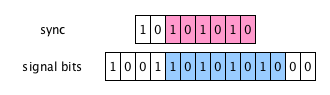
\includegraphics[width=0.45\textwidth]{figures/figure-sync-code-detection.png}
	\caption{\texttt{sync} Erkennung}
	\label{fig:sync-code-detection}
\end{wrapfigure}

Abbildung \ref{fig:sync-code-detection} skizziert das Erkennen eines Synchronisations-Codes \texttt{sync}\index{Synchronisations-Code}. Der Code wird immer mit einem Block Bits gleicher \mbox{Länge} des extrahierten Bitstroms verglichen. Die in der Skizze blau hervorgehobenen Bits sind das ein\-gebettete \texttt{sync}. Die rot markierten Bits signal\-isieren jene Zeichen, die beim \mbox{aktuellen} Vergleich über\-einstimmen. In diesem Beispiel beträgt die Über\-einstimmung zwischen er\-kanntem und tatsächlichem \texttt{sync} 75\% bei einer Synchronisation-Code Wortlänge von 8 Bit. Würde der Erkennungsschwellwert (oder \textit{Synccode-Threshold}\index{Synccode-Threshold}) ${T}_{s}$ 0.75 betragen, so wäre nun \texttt{sync} erkannt worden. Aus der Skizze ist aber ersichtlich, dass hier der tatsächlich Match erst 2 Shifts später erfolgt. Die anschließend gelesenen Informationsbits würden also teilweise aus dem Ende von \texttt{sync}\index{Synchronisations-Code} bestehen. Umgekehrt würden auch 2 echte Bits des Informationsblock\index{Information Block} nicht gelesen werden.

Das Problem in diesem Beispiel ist, dass \texttt{sync}\index{Synchronisations-Code} eine sehr hohe \textit{Autokorrelation}\index{Autokorrelation} besitzt. In anderen Worten ist \texttt{sync} (als Signal aufgefasst) sehr ähnlich zu sich selbst, weswegen 75\% Überdeckung auch zu 75\% Übereinstimmung führen. Die Lösung ist für \texttt{sync}\index{Synchronisations-Code} ein Sequenz mit minimaler Autokorrelation zu wählen. In der Literatur\cite{chang2012location}\cite{lie2006robust}\cite{huang2002blind} erfreuen sich die sog. \textit{Barker-Codes}\cite{barker1953group} großer Beliebtheit. Dabei handelt es sich um 9 Zahlensequenzen von denen der längste 13 Zeichen umfasst, welche alle die Bedingung der Autokorrelations-Funktion:

	 \begin{equation}
		 | \sum\limits_{j=1}^{N-v} a_j {a}_{j+} | \leq 1 \quad\mbox{mit}\quad 1 \leq v < N \quad\mbox{und}\quad a_j \in {-1,+1}
	 	\label{equ:barker-correlation}
	 \end{equation}

wobei $N$ die Code Länge bezeichnet, erfüllen. Es lässt sich zeigen, dass die Summe bei einer Verschiebung wie im Beispiel oben immer sehr klein ist, außer die Codes überdecken sich exakt. Gleichzeitig bleibt die Summe immer noch sehr groß (nahe an 1) wenn bei vollständiger Überdeckung innerhalb des Codes eine Zahl kippt. Ein gekipptes Bit wirkt sich also nicht so massiv auf die Erkennung des Codes aus wie eine falsche Überdeckung. Barker-Codes eignen sich daher hervorragend als Synchronisations-Code Sequenz. 

Die Länge der verwendeten Barker Sequenz wirkt sich natürlich auch auf die Erkennungsgenauigkeit aus. Hier wird der längste Barker-Code \textsf{+1 +1 +1 +1 +1 -1 -1 +1 -1 -1 +1 -1 +1} verwendet. Der Vollständigkeit halber sei noch darauf hingewiesen, dass wir nur Binärwerte kodieren können, weswegen $-1$ auf den Wert $0$ abgebildet wird. Bei der Erkennung von \texttt{sync} muss dies natürlich entsprechend bedacht werden.

Synchronisations-Codes werden genau wie die eigentlichen Informationen (die \textit{Nutzlast}) übertragen. Jeder eingebrachte \texttt{sync}\index{Synchronisations-Code} belastet daher die Transportkapazität des Signals. Es können also abhängig von der Informationsblocklänge bedeutend weniger Informationsbits effektiv in einem fixen Zeitfenster transportiert werden. 

\index{Barker-Code|)}
\index{Synchronisations-Code|)}

\subsection{Fehlerkorrekturverfahren} 
\label{sec:errorcorrection}
\index{Fehlerkorrekturverfahren|(}

Die Natur der Barker-Codes\index{Barker-Code} bringt eine gewisse Resistenz gegen Bitfehler mit sich, wie eben demonstriert wurde. Die Informationsbit haben diese im Allgemeinen nicht. Der Übertragungskanal\index{\"Ubertragungskanal} kann aber das Signal so weit beeinflussen, dass nicht alle Bits korrekt rekonstruiert werden. Es ist daher wünschenswert eine Methode zu verwenden welche derartige Bitfehler nicht nur erkennt, sondern auch korrigieren kann. Mit derartigen Modellen beschäftigt sich die \textit{Kodierungstheorie}\index{Kodierungstheorie}.

Wir verwenden hier eine Vorwärtsfehlerkorrektur\index{Vorwärtsfehlerkorrektur} (in der englischen Literator \textit{forward error correction}, daher kurz FEC) bei dem die Daten mit einem \textit{error-correcting code} \index{error-correcting code} (ECC\index{error-correcting code}) bewusst mit redundanten Daten angereichert werden. Aus dieser Redundanz lässt sich anschließend prüfen ob die Daten richtig rekonstruiert wurden und bei nicht zu starker Fehlerrate die tatsächliche Information auch wieder herstellen. 

In der Kodierungstheorie bezeichnet man mit \textit{Message}\index{Message} die Information die es zu übertragen gilt und mit \textit{Codeword}\index{Codeword} die mit Redundanz angereicherte Message. Im Informationsblock\index{\index{Information Block}} der einem jeden Synchronisations-Code\index{Synchronisations-Code} folgt befindet sich daher immer ein vollständiges Codeword um hier ggf. Übertragungsfehler auszugleichen. 

Bezeichnen wir mit $\mbox{wmk}$ das zu übertragende Watermark und mit ${L}_{w}$ seine Länge (sog. \textit{Watermark-Length}\index{Watermark-Length}, die Anzahl an Bit) dieses Watermarks, wobei $\mbox{wmk}(i)$ das Bit an der Stelle $i$ mit $i\in[1,{L}_{w}]$ referenziert, so ergeben sich folgende Bedingungen. Für die Bit-L\"ange einer Message ${L}_{m}$, genannt \textit{Message-Length}\index{Message-Length}, muss gelten:

	 \begin{equation}
		 {L}_{w} \pmod{{L}_{m}} = 0 \quad\mbox{und}\quad {L}_{w}\geq{L}_{m} 		
		 \label{equ:wmkseqlength}
	 \end{equation} 

und für die Bit-Länge eines Codewords ${L}_{c}$ (sog. \textit{Codeword-Length}\index{Codeword-Length}) gilt allgemein ${L}_{c} > {L}_{m}$
\\
Gültige Parameter für ${L}_{m}$ und ${L}_{c}$ hängen vom jeweiligen Fehlerkorrekturverfahren\index{Fehlerkorrekturverfahren} ab. Die im Folgenden angeführten Verfahren werden unterstützt:

\subsubsection{BCH-Codes}
\index{BCH-Codes}

In der Literatur\cite{chang2012location}\cite{huang2002blind} oftmals verwendet werden die nach Bose, Chaudhuri und Hocquenghem benannten BCH-Codes\cite{bose1960class}. Dabei handelt es sich um eine Gruppe von zyklischen Blockcodes um mehrere 1 Bit Fehler zu korrigieren. Es existieren verschiedene Codes und Implementierungen. Verwendet werden die System Objects \textsf{comm.BCHEncoder} und \textsf{comm.BCHDecoder} aus der MATLAB Communication System Toolbox.\footnote{\url{http://www.mathworks.de/de/help/comm/bch-codes.html}}.

\subsubsection{RS-Codes} 
\index{RS-Codes}

Reed-Solomon-Codes\cite{reed1960polynomial} (nach Irving S. Reed und Gustave Solomon) sind ebenfalls zyklischen Blockcodes, da sie eine Unterklasse der BCH-Codes sind. Ihr Prinzip ist einfach: Für eine Message\index{Message} aus $k$ Zeichen werden die $k$ Werte als Stützstellen eines Polynoms interpretiert. Mittels der Lagrange-Interpolation werden zusätzliche Stützstellen extrapoliert, sodass sich das Polynom durch $n>k$ Werte beschreiben lässt. Die $n$ Zeichen sind somit die Werte des Codewortes\index{Codeword}.

Bekannt wurden RS-Codes durch ihre Verwendung im Kommunikationsprotokoll der Voyager Sonden\footnote{Zwei interstellare Raumsonden der NASA, gestartet 1977. Beide sind heute noch aktiv (Stand 2014). Voyager 1 ist das am weitesten von der Erde entfernte, von Menschen gebaute Objekt.} und später als ECC-Verfahren\index{error-correcting code} bei CDs, DVDs, DSL oder DVB. 

Verwendet wird die MATLAB Implementierung der Communication System Toolbox\footnote{\url{http://www.mathworks.de/de/help/comm/reed-solomon-codes.html}}.

\subsubsection{LDPC-Codes}
\index{LDPC-Codes}

Low-Density-Parity-Check-Codes, von  Robert G. Gallager\cite{gallager1962low} entwickelt (daher oft auch Gallager-Codes), sind lineare ECC\index{error-correcting code} die nahe am Shannon-Limit (theoretische Obergrenze der Bitrate eines Übertragungskanals\index{\"Ubertragungskanal}) operieren. Sie sind daher ähnlich effektiv wie Turbo-Codes. Verwendung finden sie vor allem in der Fehlerkorrektur in WLAN-Standards.
Verwendet wird die MATLAB Implementierung der Communication System Toolbox\footnote{\url{http://www.mathworks.de/de/help/comm/ldpc-codes.html}}.

\index{Fehlerkorrekturverfahren|)}

\subsection{Datenstrukturen und Protokoll}
\label{sec:protokoll}
\index{Protokoll}

Jeder digitale Kommunikationsprozess basiert auf einem Protokoll welches alle Teilnehmer beherrschen müssen. So auch dieser hier, denn wenn gleich der Übertragungskanal auch analog sein mag, so werden doch digitale Daten übermittelt. Nicht nur gewährleistet ein definiertes Protokoll die korrekte Verarbeitung - die Abstrahierung erlaubt auch ein einfacheres Verständnis von Aufbau, Funktion und Zusammenspiel der einzelnen Teile. 

\begin{figure}[h]
	\centering
	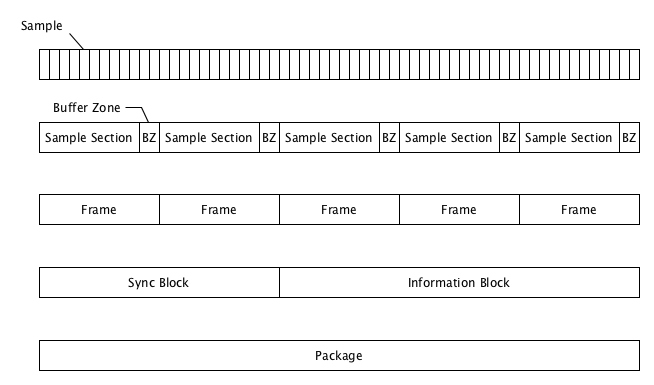
\includegraphics[width=\textwidth]{figures/figures-protocol.png}
	\caption{Hierarchischer Aufbau des Protokolls}
	\label{fig:protocol}
\end{figure}

\subsubsection{Sample Section}

Zunächst wird das Signal, welches durch zeit- und wertediskrete Samplewerten\index{Sample} beschrieben wird in Bereiche segmentiert. Es werden jeweils $N_s$\index{Sample-Section-Length} Samples\index{Sample} benötigt um 1 Bit zu transportieren. Dementsprechend werden genau die benötigte Anzahl aufeinanderfolgender Samples zu einer \textit{Sample Section} gruppiert.  

\subsubsection{Buffer Zones}
\index{Buffer Zones}

Um Interferenz zwischen den einzelnen Sample Sections\index{Sample Section} zu vermeiden befinden sich zwischen ihnen sog. \textit{Buffer Zones}. Dabei handelt es sich um eine an sich beliebige Anzahl an Samples\index{Sample}, die aber nicht zur Informationsübertragung verwendet werden. Bei der Verarbeitung der Samples werden die Buffer Zones einfach übersprungen. Prinzipiell können die Pufferzonen auch mit Sampleanzahl ${N}_{BZ} = 0$ definiert werden, allerdings führen Umweltfaktoren wie die Sensitivität des Aufnahmegerätes (und anderer AD Einflüsse \index{AD-Wandlung}) dazu, dass sich die Sample Sections überlagern\cite{chang2012location}. Das Ergebnis ist sog. \textit{Inter-Symbol-Interferenz}\footnote{Ein Symbol ist ein Element aus einem Alphabet. In binären Systemen ist das Alphabet also die Menge $\{0,1\}$.}. Die Auswirkung ist u.a. ein schlechteres Matching der Barker-Codes\index{Barker-Code} bei der Synchronisations-Code Erkennung\index{Synchronisations-Code}.

\subsubsection{Frame}
\index{Frame}

Um die Buffer Zones einfacher handzuhaben werden sie in den \textit{Frames} wegabstrahiert. Alle höheren Schichten sehen ein Frame als die logische Einheit die ein Bit transportiert. Einzig und allein die Frameverarbeitung muss über Position und Länge der Pufferzonen bescheid wissen. Für die höhere Schichten ist ein Bit in den ${N}_{F}$ Samples eines Frames, mit ${N}_{F} = {N}_{s} + {N}_{BZ}$, kodiert.

\subsubsection{Sync Block}
\index{Sync Block}

Ein Synchronisations-Code\index{Synchronisations-Code} besteht aus $L_s$\index{Synchronisations-Code-Length} Bit, daher sind ebenso viele Frames notwendig um ein \texttt{sync} zu schreiben. Diese Gruppe an Frames wird als \textit{Sync Block} bezeichnet.

\subsubsection{Information Block}
\index{Information Block}
 
Synchronisations-Codes\index{Synchronisations-Code} markieren die Stellen an denen Information vorhanden ist. Demensprechend ist jeder Sync-Block gefolgt von einem \textit{Information Block}, der sich aus $L_c$\index{Codeword-Length} aufeinander folgender Frames zusammensetzt. Ein Block transportiert immer ein vollständiges Codeword\index{Codeword}, beinhaltet somit also eine Message\index{Message} inklusive der Redundanz des ECC\index{error-correcting code}.

\subsubsection{Package}
\index{Package}

Ein Sync Block und sein Information Block bilden zusammen eine Einheit, sie existieren nie für sich alleine ohne den anderen. Demensprechend empfiehlt es sich sie in einer gemeinsamen Datenstruktur abzubilden, dem sog. \textit{Package}. Dieses eignet sich für die praktische Verwendung und lässt sich wie folgt Abbilden:


\lstset{escapechar=@,style=customc}         
\begin{lstlisting}
typedef enum { zero, one } bit_t;
typedef struct package {
    bit_t *header;
    bit_t *payload; 
} package_t;
\end{lstlisting}

Viele paketbasierte Netzwerkprotokolle definieren einen \textit{Header} (der das Packet beschreibt) und eine \textit{Payload} (die \glqq{}Nutzlast\grqq{}). Diesem entspricht auch ein Data Struct Package wenn man den Sync Block\index{Sync Block} als Header (auch wenn er nur angibt das es sich überhaupt um ein Packet handelt) und den Information Block\index{Information Block} als Payload auffasst.

Somit lässt sich der Übermittelungsprozess eines Watermarks\index{Watermark} konzeptionell beschreiben als eine Partitionierung des Watermarks in Messages geeigneter Länge (bedingt durch das Verhältnis $L_m$\index{Message-Length} zu $L_c$\index{Codeword-Length} des ECC\index{error-correcting code}) und deren Versand durch Pakete.

\subsubsection{Parallelen zum OSI-Modell}

Vergleicht man dieses Protokoll mit dem OSI-Modell\index{OSI-Modell}\footnote{\textit{Open Systems Interconnection Model}, auch ISO-OSI-Modell. Ein Netzwerkprotokolle mit Schichtenarchitektur. Früher tatsächlich in Verwendung, wird heute vor allem als Referenzmodell herangezogen.} so erkennt man folgendes: Frames\index{Frame} (und somit auch Sample Sections und Buffer Zones) sind hier Teil des \textit{Physical Layer} (Schicht 1), welcher sich um die Bitübertragung kümmert. Packages und deren Sync bzw. Information Blocks kümmern sich um  die Segmentierung von Bitdatenströmen in Blöcke und die Kanalkodierung. Sie bilden daher den \textit{Data Link Layer} (Schicht 2) ab.
 
\subsection{Qualitätskontrolle}
\label{sec:qualitaetskontrolle}
\index{Qualitätskontrolle|(}

Das Einbringen des Watermarks\index{Watermark} unterlieg der Bedingung, dass es unhörbar (für den Menschen) sein soll. Um dies zu gewährleisten muss jedes bearbeitete Teilstück des Signals einer Qualitätskontrolle diesbezüglich unterzogen werden. Dazu existieren prinzipiell folgende Methoden:

\subsubsection{Mean Opinion Score}
\index{Mean Opinion Score}

Definiert in der ITU-T Recommendation P.800\cite{rec1996p} handelt es sich beim \textit{Mean Opinion Score} (MOS) um das Ergebnis der Bewertungen einer Reihe von subjektiven Wahrnehmungstest durch Versuchspersonen. Damit werden die Qualitäten von Codecs in der Sprach- und Bildübertragung bewertet. Da hierfür jedes Segment einzeln von menschlichen Versuchspersonen als Teil des Algorithmus behandelt werden müsste, eignet es sich ganz offensichtlich nicht für eine automatische Verarbeitung. 

\subsubsection{Signal-Rauschabstand} 
\index{Signal-Rauschabstand}

Der Signal-Rauschabstand oder Signal-Rausch-Verhältnis (engl. \textit{signal-to-noise ratio}, daher kurz SNR) bewertet die technische Qualität eines Signals welches von einem Störsignal überlagert wird. Hier ist zu beachten, dass mit Störsignal nicht jenes im analogen Übertragungskanal\index{\"Ubertragungskanal} gemeint ist. Die Veränderung eines Audiosignals durch das Watermark\index{Watermark} kann bezogen auf das ursprünglich unmodifizierte Signal ebenfalls als Störsignal interpretiert werden. 

Der SNR berechnet sich durch: 
	\begin{equation}	
		\mbox{SNR} = {\mbox{Nutzsignalleistung} \over \mbox{Rauschsignalleistung}},
		\label{equ:snr}
	\end{equation}

seine Bestimmung ist daher sehr einfach. Leider handelt es sich dabei um eine technisch objektive Güteeigenschaft die das menschliche Hörsystem nicht mit einbezieht und daher als Bewertungskriterium dementsprechend schlecht geeignet ist\cite{xiang2007robust}.

\subsubsection{Objective Difference Grade} 
\index{Objective Difference Grade}
\index{Perceptual Evaluation of Audio Quality}

Offensichtlich ist es als notwendig ein automatisch berechenbares Qualitätskriterium heranzuziehen, welches allerdings eine auf die menschliche Wahrnehmung skalierte Bewertungsmetrik abbildet. Genau hierfür wurde 1998 die ITU Recommendation BS.1387\cite{rec1998bs}, besser bekannt als \textit{Perceptual Evaluation of Audio Quality} (PEAQ) spezifiziert. Mit ihr lässt sich für ein Audiosignal der sog. \textit{Objective Difference Grade} (ODG) berechnen, ein Wert im Intervall $[-4,0]$ wobei $0$ für  \glqq{}unhörbar\grqq{} und $-4$ für \glqq{}sehr störend\grqq{} steht. Es hat sich gezeigt, dass die Korrelation von PEAQ Bewertung und MOS ca. 0.98 beträgt\cite{al2011dwt}.

Leider hat sich recht bald herausgestellt, dass die Berechnung des ODGs nicht hinreichend genau spezifiziert ist\cite{kabal2002examination}\cite{campeanu2005peaq}, was sich auch in der Qualität der derzeit vorhandenen Tools wiederspiegelt. Eine kurze Evaluierung gängiger PEAQ Implementierungen findet sich in Anhang \ref{ch:peaq}.

\index{Qualitätskontrolle|)}

\newpage

\section{Watermark Extrahierung}
\label{sec:extraction}

Nachdem das Watermark\index{Watermark} nach den nun beschriebenen Schritten in ein Signal eingebettet und anschließend übertragen wurde, gilt es nun die Informationsdaten wieder zu extrahieren. Abbildung \ref{fig:diagram-decoder} zeigt den schematischen Ablauf des Dekodierungsprozesses.

\begin{figure}[h]
	\centering
	%\includesvg[width=0.7\textwidth]{figures/diagram-framework.svg}
	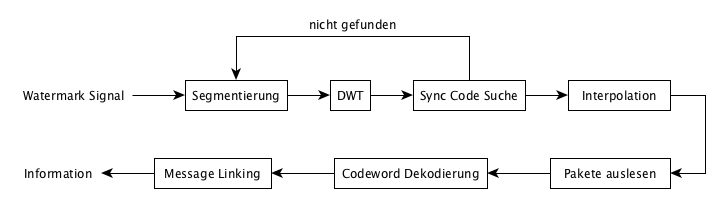
\includegraphics[width=0.9\textwidth]{figures/diagram-decoder-v2.png}
	\caption{Schematischer Aufbau des Extraktionsprozesses}
	\label{fig:diagram-decoder}
\end{figure}


\subsection{Resynchronisaton und Interpolation}

Bei der Erkennung der Synchronisations-Codes kann es im Allgemeinen zu Problemen kommen. Die bei der DA-Wandlung\index{DA-Wandlung} auftretenden Einflüssen lassen sich im Allgemeinen durch eine Kombination aus \textit{time scaling modification}\index{time scaling modification} (kurz TSM, dt. interessanterweise bekannt als \textit{Time-Stretching}) und \index{wave magnitude
distortion}\textit{wave magnitude
distortion} (WMD) beschreiben\cite{xiang2007robust}\cite{steinebach2002audio}. Die TSM kann das Auffinden der Synchronisation-Codes verhindern. Das Prinzip kann daher auch gezielt eingesetzt werden, um ein existierendes Watermark\index{Watermark} zu zerstören (etwa um einen Urheberrechtlichsschutz aufzuheben). Dies wird als \textit{Synchronization attack}\index{Synchronization attack} bezeichnet.

Um diesen Effekt der DA-Wandlung\index{DA-Wandlung} aufzuheben, muss versucht werden die Synchron\-isations\--Codes wieder\-herzustellen. Man nennt diesen Vorgang \textit{Resynchronisation}\index{Resynchronisation}. Verschiedene Resynchronisationsansätze existieren, hier wird ein sog. \textit{brute-force approach}\index{brute-force approach} angewandt und wie in \cite{steinebach2011re} vorgeschlagen auf ein Suchintervall von -10\% bis +10\% beschränkt. 

Die TSM bewirkt, dass das Signal auf seiner Zeitachse gestreckt oder gestaucht wird. Für das Watermark\index{Watermark} bedeutet das, dass ein Bit nicht mehr in $N_s$\index{Sample-Section-Length} Samples kodiert ist, sondern durch mehr oder weniger Samples ${N}_{s}'$ beschrieben wird. 
Zuerst gilt es die neue Sampleanzahl ${N}_{s}'$ zu finden. Dazu wird ${N}_{s}'$ von $0.9 \cdot {N}_{s}$ bis $1.1 \cdot {N}_{s}$ durchgetestet und nach Synchronisations-Codes\index{Synchronisations-Code} gesucht. Algorithmus \ref{alg:resync} illustriert diesen Vorgang.

\RestyleAlgo{algoruled}
\begin{algorithm}[h]

	\SetKwData{Framelen}{framelen}
	\SetKwData{Ns}{${N}_{s}$}
	\SetKwData{Steplen}{steplen}
	\SetKwData{Upperbound}{upperbound}
	\SetKwData{Lowerbound}{lowerbound}
	\SetKwData{Sig}{sig}
	\SetKwData{Size}{size}
	\SetKwData{Testwindow}{testwindow}
	\SetKwData{Cursor}{cursor}
	\SetKwData{Found}{found}
	\SetKwFunction{Resynchronize}{resynchronize}
	\SetKwFunction{Testsync}{testsync}
	\SetKwInOut{Input}{input}
	\SetKwInOut{Output}{output}

\Input{Samples eines Signals}
\Output{Resynchronisiertes Signal}

\BlankLine

\Steplen = 0.005 * \Ns\;
\Lowerbound = 0.9 * \Ns\;
\Upperbound = 1.1 * \Ns\;
\Cursor = 1\;

\While{ \Cursor < \Size - \Upperbound and not \Found }{
	\Framelen = \Lowerbound\;
	\While{\Framelen < \Upperbound}{
		\Testwindow = \Sig[\Cursor,\Framelen]\;
		\Found = \Testsync{\Testwindow}\;
		\eIf{\Found}{ 
			\Resynchronize{\Sig,\Framelen}\;
		}{ 
			\Framelen = \Framelen + \Steplen\;
		}
	}
	\Cursor = \Cursor + 0.1 * \Lowerbound\; 
}
\caption{\texttt{sync} Erkennung in der Resynchronisationsphase}
\label{alg:resync}
\end{algorithm}


Wurde ein \texttt{sync}\index{Synchronisations-Code} gefunden, so kann man das Verhältnis zwischen neuer und alter Sampleanzahl

	\begin{equation}
		\alpha = { {N}_{s}' \over {N}_{s} }
		\label{equ:resampling_factor}
	\end{equation}
	\index{Sample-Section-Length}

berechnet werden. Mit $\alpha$ können nun alle Samples als Vorverarbeitungsschritt auf ihren ursprünglichen Wert rückinterpoliert werden. Verschiedene Interpolationsverfahren führen hier zu keinem merklichen Unterschied\cite{xiang2007robust}, weswegen eine lineare Lagrange-Interpolation\index{Lagrange-Interpolation} verwendet wird. Somit können die neuen Samplewerte $f''(i)$ durch

	\begin{equation}
		f''(i) = \begin{cases}
    	 	f'(i) & \iff i = 1	
			\\
			(1-\beta) \cdot f'(\lfloor\alpha \cdot i\rfloor) + \beta \cdot f'(\lfloor\alpha \cdot i\rfloor + 1) & \iff 1 < i < {N}_{s} 
			\\
    		f({N}_{s}') & \iff i = {N}_{s}
  		 \end{cases}
		\label{equ:lagrange_interpolation}
	\end{equation}
	
wobei $f'(i)$ die alten Werte und $\beta = \alpha \cdot i - \lfloor \alpha \cdot i \rfloor$ beschreibt, berechnet werden. Somit kann für die Extrahierung das exakt selbe Verfahren zur Analyse der DWT-Koeffizienten\index{DWT-Koeffizienten} wie im Implantationsprozess verwendet werden. 

\subsection{Datenextrahierung}

Nach der Resynchronisation kann das Signal schrittweise durchlaufen und nach \texttt{sync} Sequenzen gescannt werden. Dabei wird das Signal genau so wie in der Implementierungsphase in Samples Sections zerteilt, die DWT-Koeffizienten für die Samples berechnet und nach dem Prinzip aus Kapitel \ref{sec:reconstruction} für jedes Segment ein binärer Wert bestimmt. Anschließend werden immer $L_s$\index{Synchronisations-Code-Length} aufeinander folgende Binärwerte auf ihre Übereinstimmung mit dem Synchronisations-Code\index{Synchronisations-Code} \texttt{sync} überprüft.

Erfolgt ein Match auf den Synchronisations-Code, so sind die folgenden $L_c$\index{Codeword-Length} Bit als Informationsbits aufzufassen. Da es sich um ein Codeword\index{Codeword} handelt, muss noch der Dekodierungsalgorithmus des ECC\index{error-correcting code} angewendet werden, um die Message\index{Message} zu erhalten. Die einzelnen Messages ergeben schließlich zusammengesetzt die eigentliche Information. 

Wie man sich anhand der Abbildung \ref{fig:protocol} leicht überlegen kann, können immer nachdem ein Codeword erfolgreich gelesen wurde die folgenden $L_c$\index{Codeword-Length} Samples Sections \index{Sample Section} auf der Suche nach weiteren \texttt{sync}\index{Synchronisations-Code} Sequenzen übersprungen werden.




